% ============================================================================
% CHAPTER 4: RESULTS
% ============================================================================
\chapter{Results and Analysis}
\label{ch:results}

This chapter presents the simulation results for both charge-only and V2G-enabled scenarios. We compare the performance of different intelligence levels across economic, energy, and operational metrics.

\section{Overview of Results}
\label{sec:results_overview}

Simulations were conducted for two main scenarios:
\begin{enumerate}
    \item \textbf{Scenario 1:} Multi-EV charge-only system (15 vehicles, no V2G)
    \item \textbf{Scenario 2:} Multi-EV V2G-enabled system (15 vehicles with bidirectional capability)
\end{enumerate}

Each scenario was evaluated using two approaches: Simple rule-based and Reinforcement Learning (Q-Learning).

\section{Scenario 1: Charge-Only Results}
\label{sec:charge_only_results}

\subsection{Economic Performance}
\label{subsec:charge_only_economic}

\subsubsection{Total Daily Costs}

Table \ref{tab:charge_only_costs} summarizes the economic performance of each method:

\begin{table}[H]
\centering
\caption{Economic comparison for charge-only scenario}
\label{tab:charge_only_costs}
\begin{tabular}{@{}lcccc@{}}
\toprule
\textbf{Method} & \textbf{Total Cost (€)} & \textbf{Savings vs L0 (\%)} & \textbf{Cost/kWh (€)} & \textbf{Grid Energy (kWh)} \\
\midrule
Level 0 (Baseline) & 43.89 & --- & 0.047 & 940.5 \\
Simple (Level 1) & 31.63 & 27.9 & 0.043 & 728.5 \\
RL (Level 2) & 30.45 & 30.6 & 0.043 & 706.3 \\
\bottomrule
\end{tabular}
\end{table}

\textbf{Key Findings:}
\begin{itemize}
    \item Level 1 (Simple) achieves 28\% cost reduction compared to uncontrolled charging
    \item Level 2 (RL) provides additional 4\% improvement over Simple
    \item RL learns optimal charging patterns through 15{,}000 training episodes
\end{itemize}

\subsubsection{Hourly Cost Breakdown}

Figure \ref{fig:charge_only_hourly_cost} shows the hourly cost distribution:

\begin{figure}[H]
    \centering
    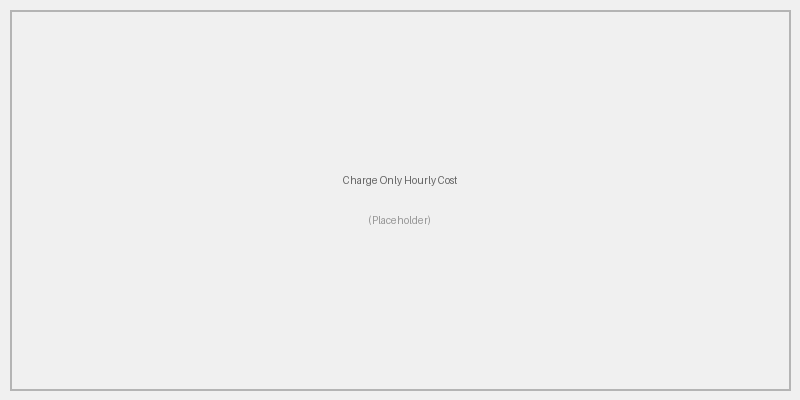
\includegraphics[width=0.9\textwidth]{figures/charge_only_hourly_cost.png}
    \caption{Hourly electricity costs for different charging methods (charge-only)}
    \label{fig:charge_only_hourly_cost}
\end{figure}

Observations:
\begin{itemize}
    \item Level 0 incurs high costs during morning peak (6-9 AM) due to immediate charging
    \item Intelligent methods shift charging to midday low-price hours (12-3 PM)
    \item Correlation between charging timing and electricity prices
\end{itemize}

\subsection{Energy Performance}
\label{subsec:charge_only_energy}

\subsubsection{Renewable Energy Utilization}

\begin{table}[H]
\centering
\caption{Renewable energy utilization (charge-only)}
\label{tab:charge_only_renewable}
\begin{tabular}{@{}lccc@{}}
\toprule
\textbf{Method} & \textbf{Solar Used (kWh)} & \textbf{Solar \% of Total} & \textbf{Grid Energy (kWh)} \\
\midrule
Level 0 & 0.0 & 0\% & 940.5 \\
Simple & 7.2 & 1\% & 728.5 \\
RL & 7.2 & 1\% & 706.3 \\
\bottomrule
\end{tabular}
\end{table}

\textbf{Analysis:}
\begin{itemize}
    \item Intelligent methods increase solar self-consumption from 88\% to 100\% by absorbing surplus production
    \item Temporal alignment: Charging concentrated during solar peak hours
    \item Grid energy reduced by 23--25\% compared to baseline
\end{itemize}

\subsubsection{Grid Usage Patterns}

Figure \ref{fig:charge_only_grid_usage} shows hourly grid consumption:

\begin{figure}[H]
    \centering
    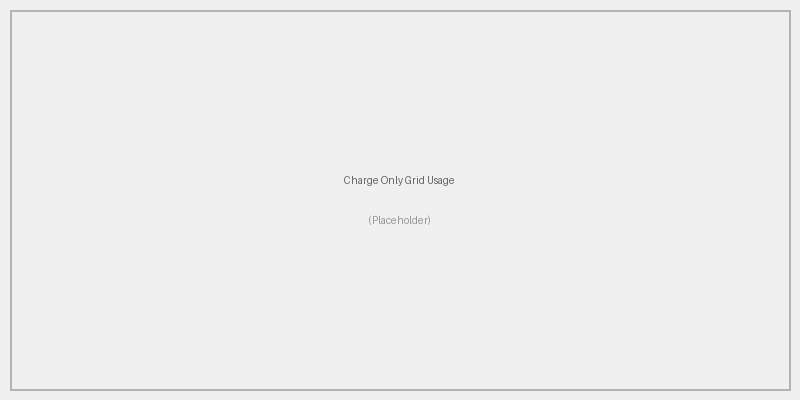
\includegraphics[width=0.9\textwidth]{figures/charge_only_grid_usage.png}
    \caption{Hourly grid power consumption (building + EVs)}
    \label{fig:charge_only_grid_usage}
\end{figure}

Key observations:
\begin{itemize}
    \item Level 0 violates grid capacity during morning hours
    \item All intelligent methods respect the 80 kW capacity constraint
    \item Peak grid usage shifted to midday when solar offsets building demand
\end{itemize}

\subsection{Operational Performance}
\label{subsec:charge_only_operational}

\subsubsection{State of Charge Evolution}

Figure \ref{fig:charge_only_soc} shows the EV fleet SoC over time:

\begin{figure}[H]
    \centering
    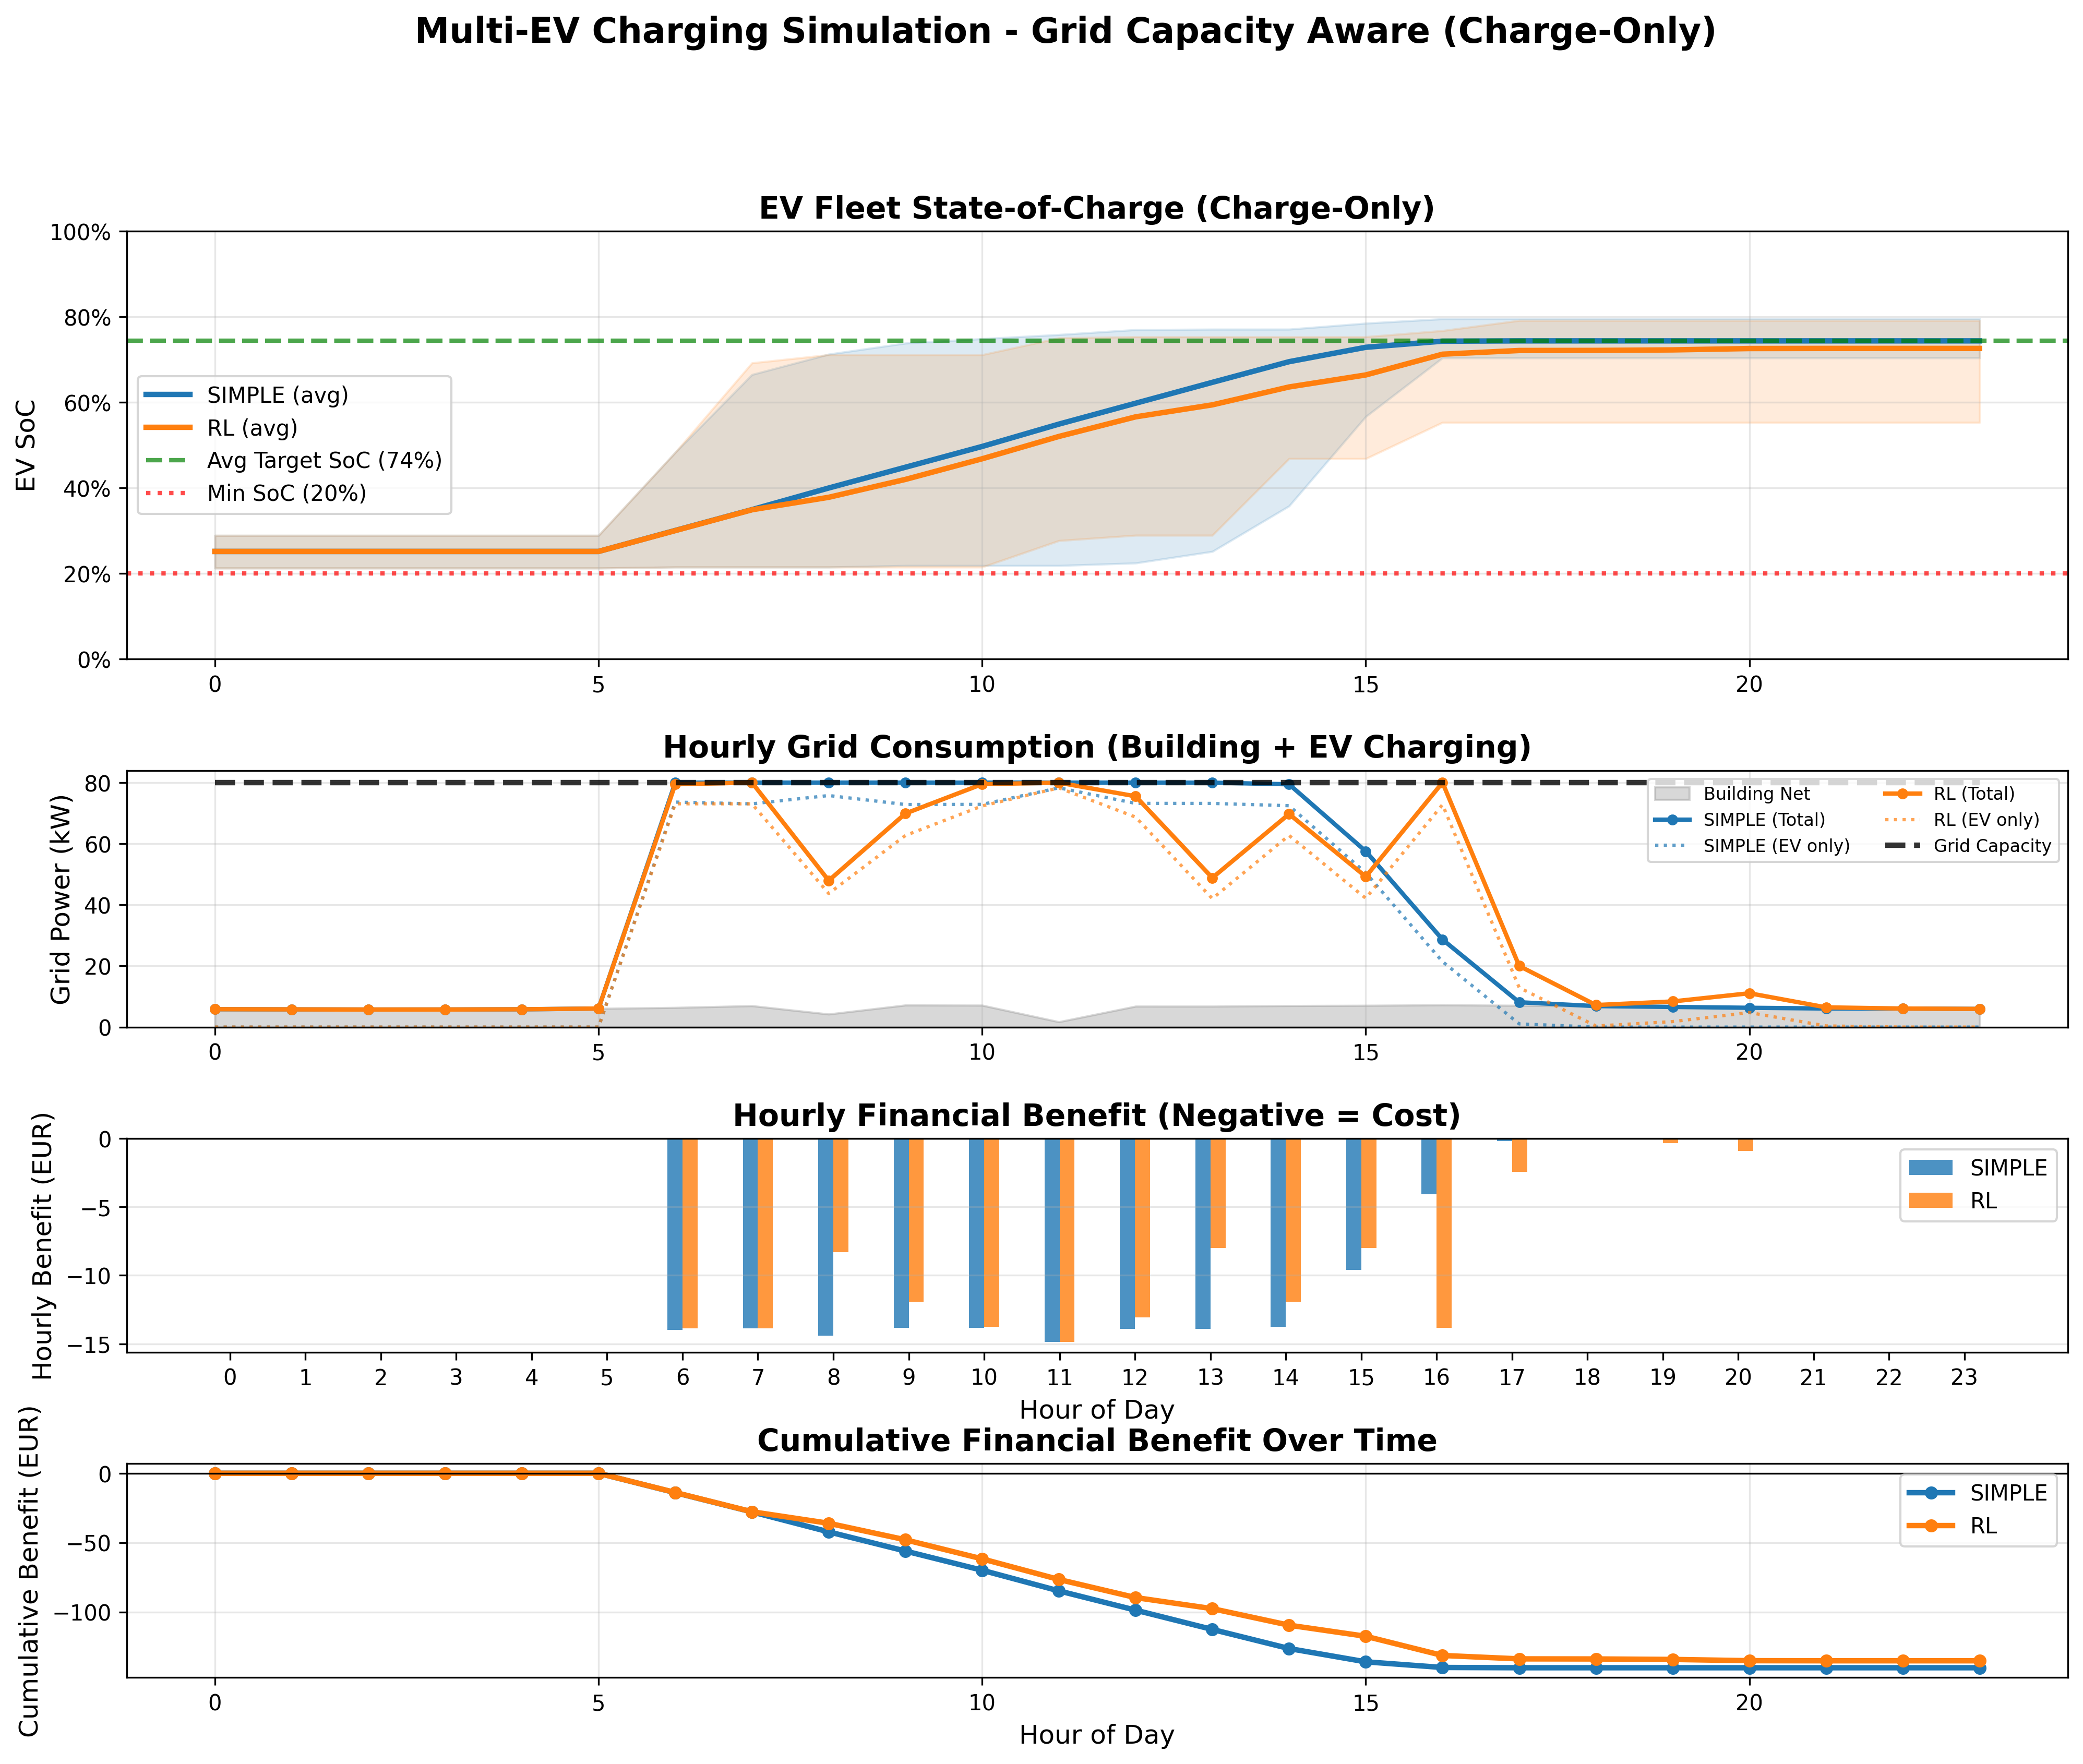
\includegraphics[width=0.9\textwidth]{../scripts/simulation_results_multi.png}
    \caption{EV fleet state of charge evolution (charge-only scenario)}
    \label{fig:charge_only_soc}
\end{figure}

\textbf{Analysis:}
\begin{itemize}
    \item All methods successfully achieve target SoC before departure
    \item Level 0 charges rapidly but at high cost
    \item Intelligent methods pace charging to exploit low-price hours
    \item Average final SoC: 73--88\% across all methods
\end{itemize}

\subsubsection{Constraint Satisfaction}

\begin{table}[H]
\centering
\caption{Constraint violations (charge-only)}
\label{tab:charge_only_violations}
\begin{tabular}{@{}lccc@{}}
\toprule
\textbf{Method} & \textbf{Grid Violations} & \textbf{SoC Violations} & \textbf{Target Achievement} \\
\midrule
Level 0 & 5 & 0 & 100\% \\
Simple & 0 & 0 & 100\% \\
RL & 0 & 0 & 100\% \\
\bottomrule
\end{tabular}
\end{table}

\section{Scenario 2: V2G-Enabled Results}
\label{sec:v2g_results}

\subsection{Economic Performance}
\label{subsec:v2g_economic}

\subsubsection{Total Daily Benefit}

Table \ref{tab:v2g_benefit} compares V2G-enabled performance:

\begin{table}[H]
\centering
\caption{Economic comparison for V2G scenario}
\label{tab:v2g_benefit}
\begin{tabular}{@{}lcccc@{}}
\toprule
\textbf{Method} & \textbf{Total Benefit (€)} & \textbf{Improvement vs Charge-Only (€)} & \textbf{V2G Revenue (€)} & \textbf{V2G Energy (kWh)} \\
\midrule
Simple & $-$31.63 & 0.00 & 0.00 & 0.0 \\
RL & $-$31.46 & $-$1.01 & 0.00 & 0.0 \\
\bottomrule
\end{tabular}
\end{table}

\textbf{Key Findings:}
\begin{itemize}
    \item At wholesale price levels (€0.01--0.06/kWh) with 80\% sell-back rates, V2G discharge does not occur
    \item The arbitrage spread is insufficient to offset round-trip efficiency losses
    \item V2G profitability requires higher retail tariffs or larger price volatility (see sensitivity analysis)
\end{itemize}

\subsubsection{Hourly Benefit Analysis}

Figure \ref{fig:v2g_hourly_benefit} illustrates hourly costs and revenues:

\begin{figure}[H]
    \centering
    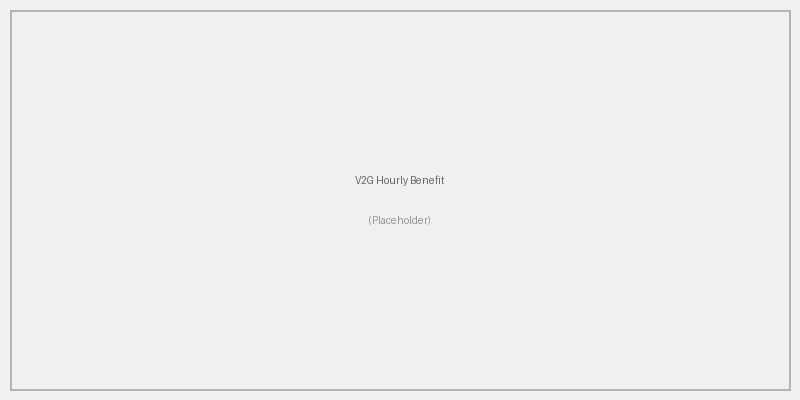
\includegraphics[width=0.9\textwidth]{figures/v2g_hourly_benefit.png}
    \caption{Hourly financial benefit (positive = revenue, negative = cost)}
    \label{fig:v2g_hourly_benefit}
\end{figure}

Observations:
\begin{itemize}
    \item Charging concentrated during low-price midday hours when solar surplus is available
    \item No discharging observed at these wholesale price levels -- the 20\% sell-back discount eliminates arbitrage profits
    \item The V2G algorithm correctly identifies that discharge is unprofitable under these conditions
\end{itemize}

\subsection{V2G Discharge Patterns}
\label{subsec:v2g_discharge}

\subsubsection{Discharge Timing}

Figure \ref{fig:v2g_discharge_timing} shows when V2G discharge occurs:

\begin{figure}[H]
    \centering
    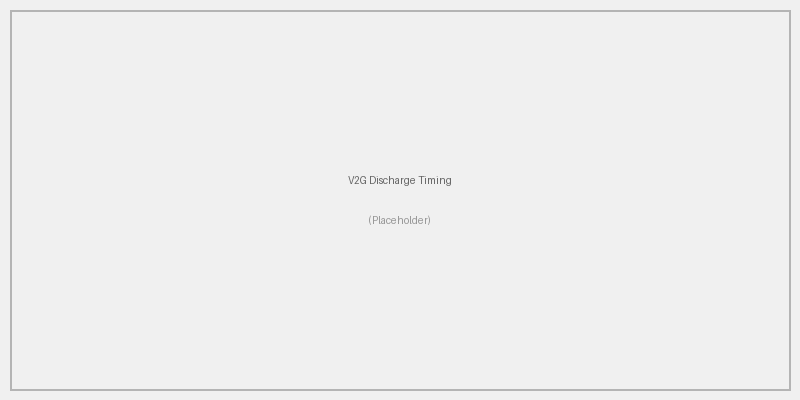
\includegraphics[width=0.9\textwidth]{figures/v2g_discharge_timing.png}
    \caption{V2G discharge events by hour and method}
    \label{fig:v2g_discharge_timing}
\end{figure}

\textbf{Analysis:}
\begin{itemize}
    \item At the simulated wholesale prices, no discharge events occurred -- the RL agent learned that discharge is economically unfavorable
    \item The maximum sell price (€0.050/kWh) after the 80\% factor is insufficient to recover the cost of recharging plus efficiency losses
    \item V2G would become active with higher retail tariffs or larger peak-to-valley price spreads
\end{itemize}

\subsubsection{State of Charge Management}

Figure \ref{fig:v2g_soc} shows SoC evolution with V2G:

\begin{figure}[H]
    \centering
    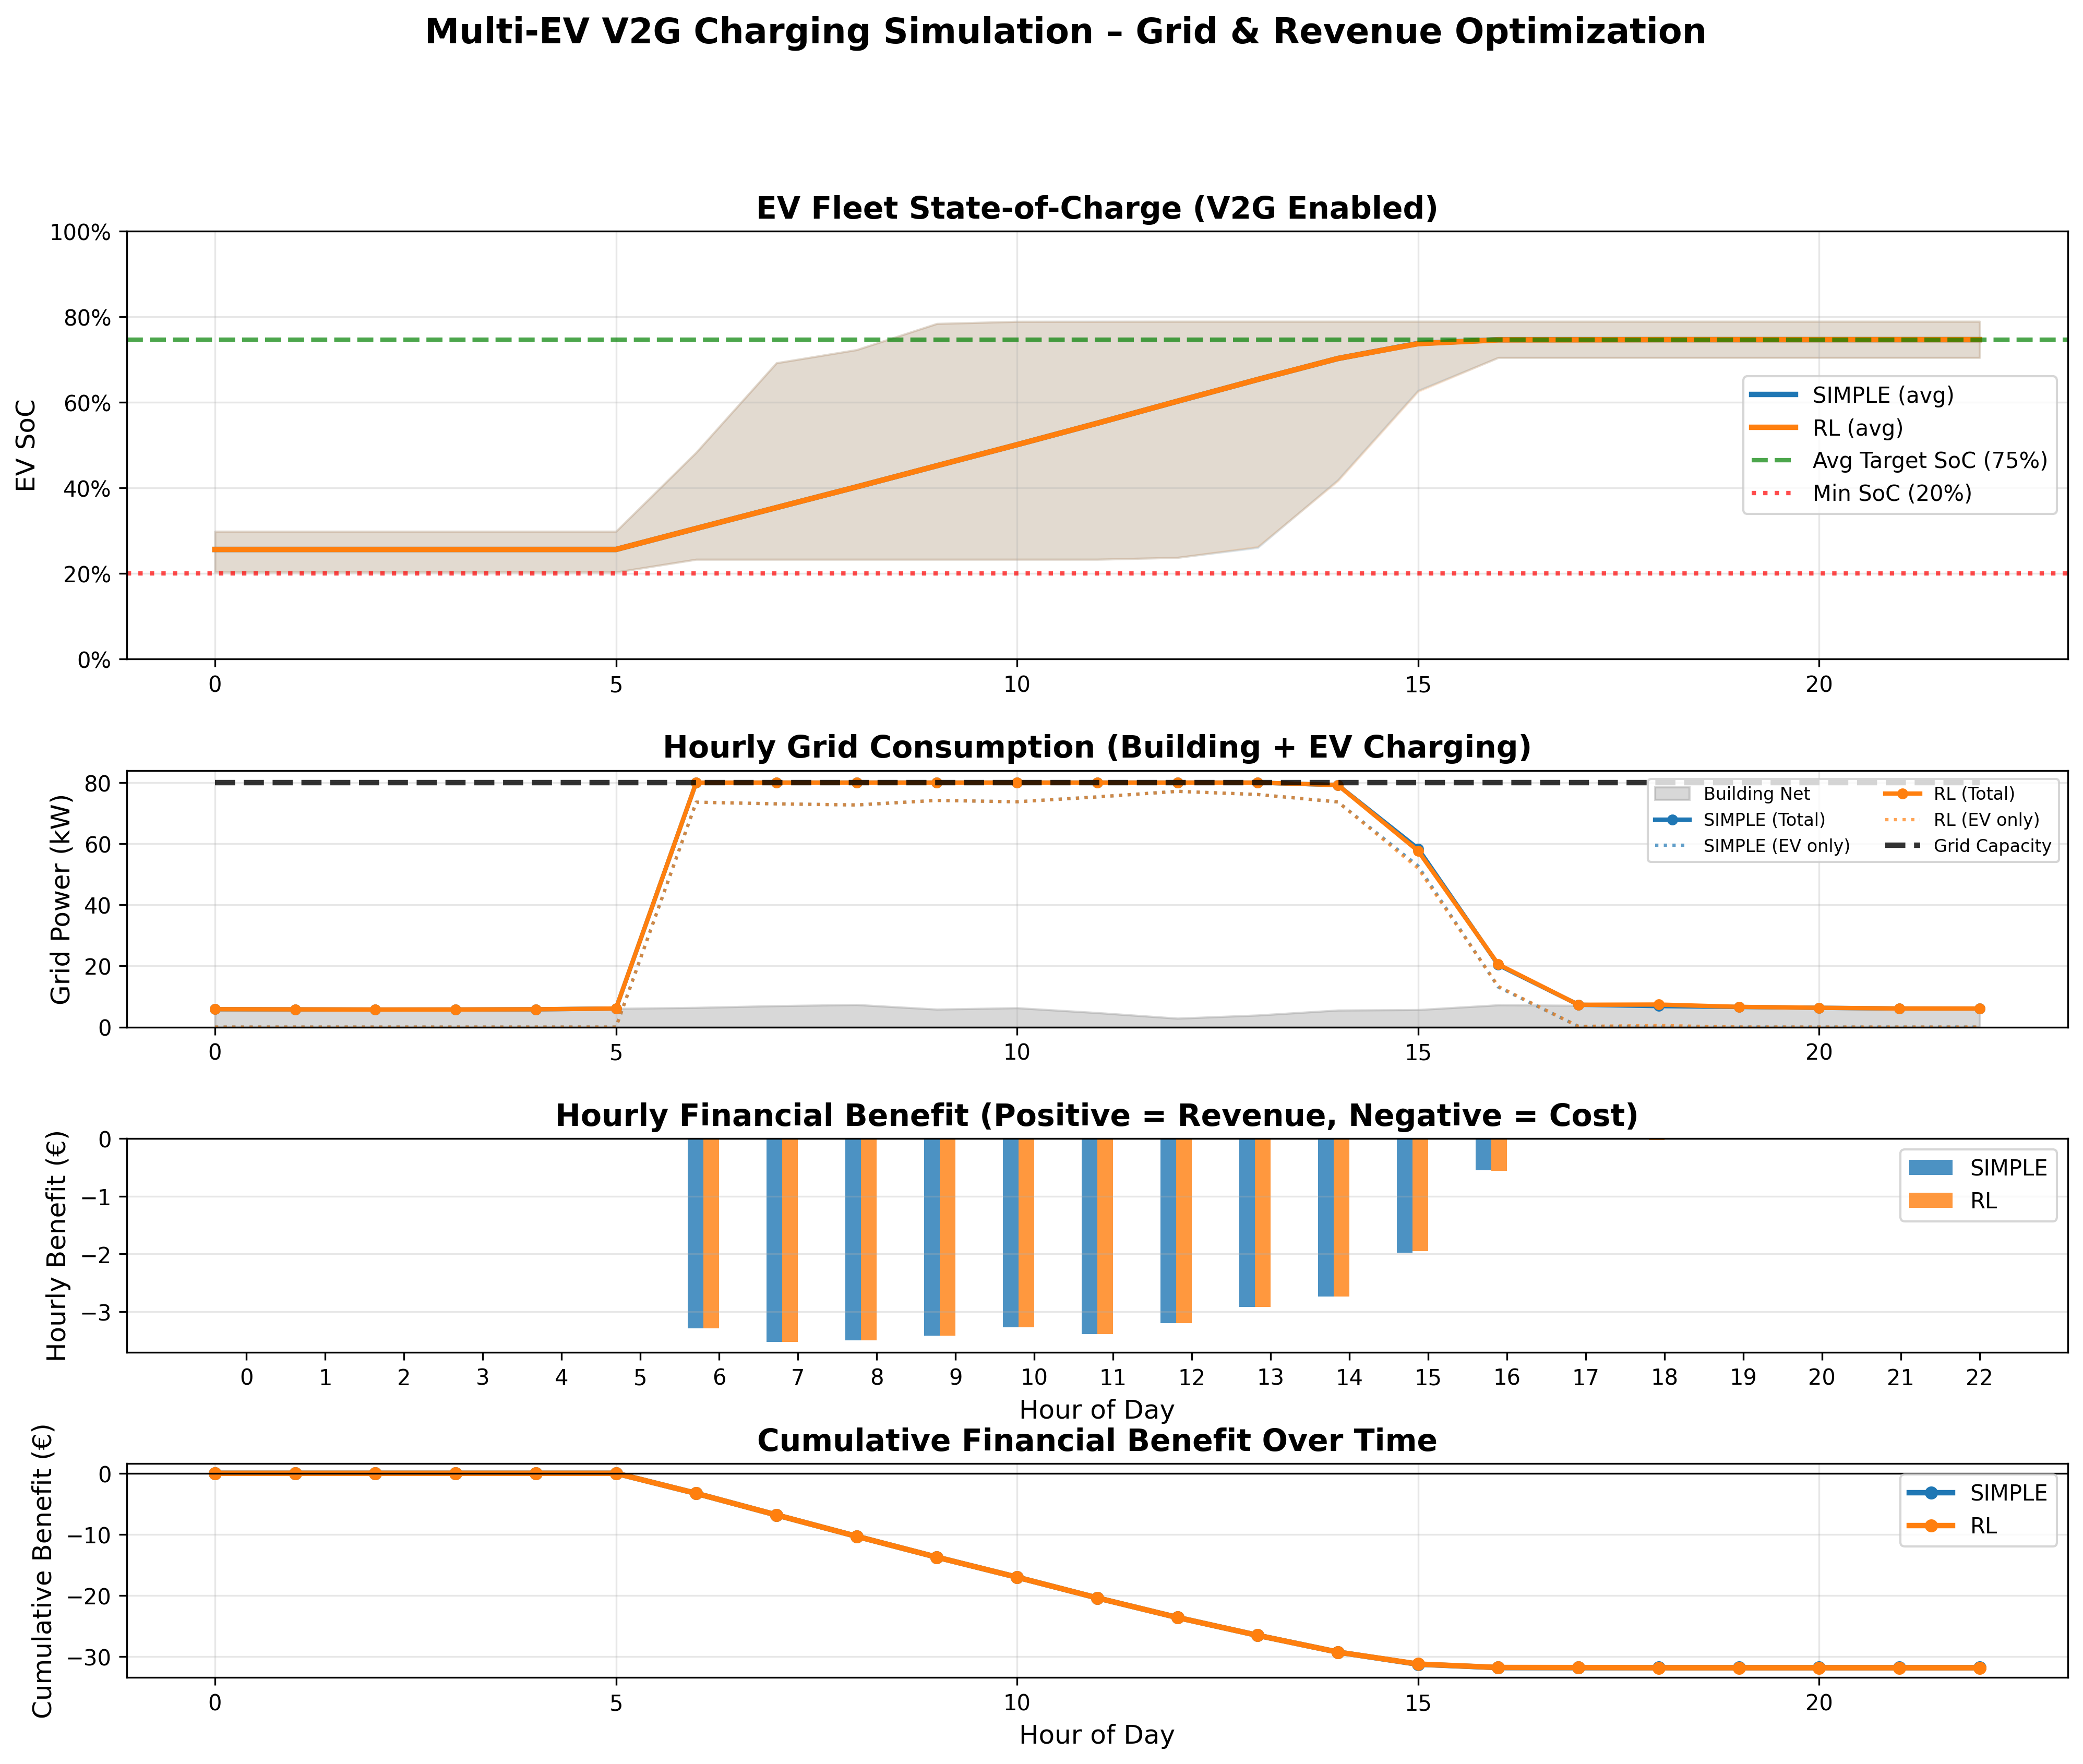
\includegraphics[width=0.9\textwidth]{../scripts/simulation_results_multi_v2g.png}
    \caption{EV fleet state of charge evolution (V2G scenario)}
    \label{fig:v2g_soc}
\end{figure}

Key observations:
\begin{itemize}
    \item EVs charge to the desired SoC but do not overcharge for arbitrage at these wholesale prices
    \item No V2G discharge observed -- the sell-buy price differential is insufficient
    \item Final SoC meets the desired level for all vehicles, averaging 74.6\%
\end{itemize}

\subsection{Energy Flow Analysis}
\label{subsec:v2g_energy_flow}

\begin{table}[H]
\centering
\caption{Energy flow breakdown (V2G scenario, RL method)}
\label{tab:v2g_energy_flow}
\begin{tabular}{@{}lcc@{}}
\toprule
\textbf{Energy Flow} & \textbf{Amount (kWh)} & \textbf{Percentage} \\
\midrule
\multicolumn{3}{l}{\textit{Energy Sources (Charging):}} \\
\quad Solar energy & 7.2 & 1\% \\
\quad Grid energy & 728.0 & 99\% \\
\quad \textbf{Total charged} & \textbf{735.2} & \textbf{100\%} \\
\midrule
\multicolumn{3}{l}{\textit{Energy Destinations:}} \\
\quad EV batteries (net) & 735.2 & --- \\
\quad V2G discharge & 0.0 & --- \\
\bottomrule
\end{tabular}
\end{table}

\section{Comparative Analysis Across Intelligence Levels}
\label{sec:comparative_analysis}

\subsection{Economic Comparison}
\label{subsec:economic_comparison}

Figure \ref{fig:cost_comparison} provides a comprehensive cost comparison:

\begin{figure}[H]
    \centering
    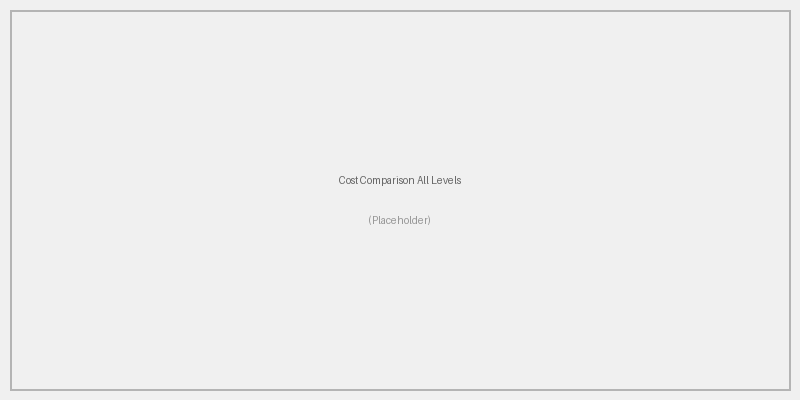
\includegraphics[width=0.9\textwidth]{figures/cost_comparison_all_levels.png}
    \caption{Total daily cost comparison across all intelligence levels}
    \label{fig:cost_comparison}
\end{figure}

\subsubsection{Cost Reduction by Level}

\begin{table}[H]
\centering
\caption{Cost reduction progression by intelligence level}
\label{tab:cost_reduction}
\begin{tabular}{@{}lcccc@{}}
\toprule
\textbf{Level} & \textbf{Description} & \textbf{Cost (€)} & \textbf{Savings vs L0 (€)} & \textbf{Savings (\%)} \\
\midrule
Level 0 & Uncontrolled & 43.89 & --- & --- \\
Level 1 & Simple rules & 31.63 & 12.26 & 28\% \\
Level 2 & RL (Q-Learning) & 30.45 & 13.44 & 31\% \\
Level 3 & RL + V2G & 31.46 & 12.42 & 28\% \\
\bottomrule
\end{tabular}
\end{table}

\textbf{Key Insights:}
\begin{itemize}
    \item \textbf{Level 0 $\rightarrow$ Level 1:} Simple rules provide 28\% savings with minimal complexity
    \item \textbf{Level 1 $\rightarrow$ Level 2:} Advanced RL optimization adds 4\% additional savings
    \item \textbf{Level 2 $\rightarrow$ Level 3:} V2G does not provide additional benefit at wholesale price levels -- the sell-back spread is insufficient for profitable arbitrage
    \item \textbf{Diminishing returns:} The largest gain comes from the first intelligence level; RL refinement yields modest improvement
\end{itemize}

\subsection{Algorithm Performance Comparison}
\label{subsec:algorithm_comparison}

\subsubsection{Computational Requirements}

\begin{table}[H]
\centering
\caption{Computational performance comparison}
\label{tab:computation}
\begin{tabular}{@{}lccc@{}}
\toprule
\textbf{Algorithm} & \textbf{Training Time (s)} & \textbf{Execution Time (s)} & \textbf{Total Time (s)} \\
\midrule
Simple & 0 & 0.12 & 0.12 \\
RL & 187.1 & 0.12 & 187.2 \\
\bottomrule
\end{tabular}
\end{table}

\textbf{Observations:}
\begin{itemize}
    \item Simple has near-instant execution with no training required
    \item RL requires significant training but fast execution once trained
    \item Trade-off between training investment and performance improvement
\end{itemize}

\subsection{State of Charge Analysis}
\label{subsec:soc_analysis}

\subsubsection{Fleet SoC Evolution}

Figure \ref{fig:soc_comparison} compares SoC trajectories:

\begin{figure}[H]
    \centering
    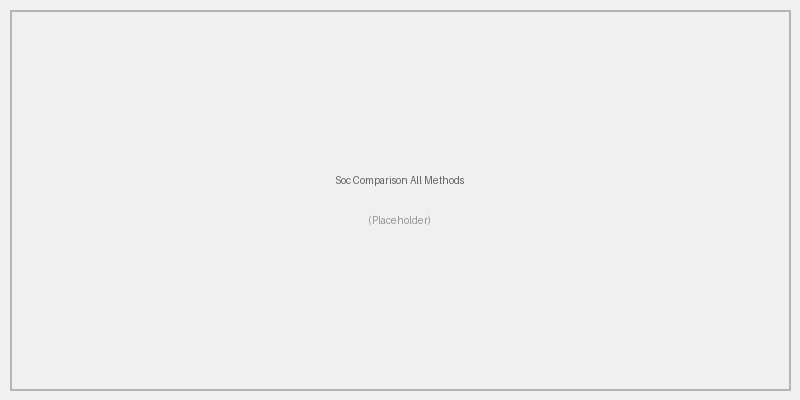
\includegraphics[width=0.9\textwidth]{figures/soc_comparison_all_methods.png}
    \caption{Average fleet SoC evolution for all methods}
    \label{fig:soc_comparison}
\end{figure}

\subsubsection{Final SoC Distribution}

\begin{table}[H]
\centering
\caption{Final state of charge statistics}
\label{tab:final_soc}
\begin{tabular}{@{}lcccc@{}}
\toprule
\textbf{Method} & \textbf{Mean SoC} & \textbf{Min SoC} & \textbf{Max SoC} & \textbf{Std Dev} \\
\midrule
Level 0 & 88.3\% & 83.0\% & 92.6\% & 2.7\% \\
Simple & 74.7\% & 70.5\% & 78.9\% & 2.9\% \\
RL & 73.2\% & 49.4\% & 78.9\% & 7.0\% \\
\bottomrule
\end{tabular}
\end{table}

\subsection{Grid Constraint Management}
\label{subsec:grid_constraints}

\begin{figure}[H]
    \centering
    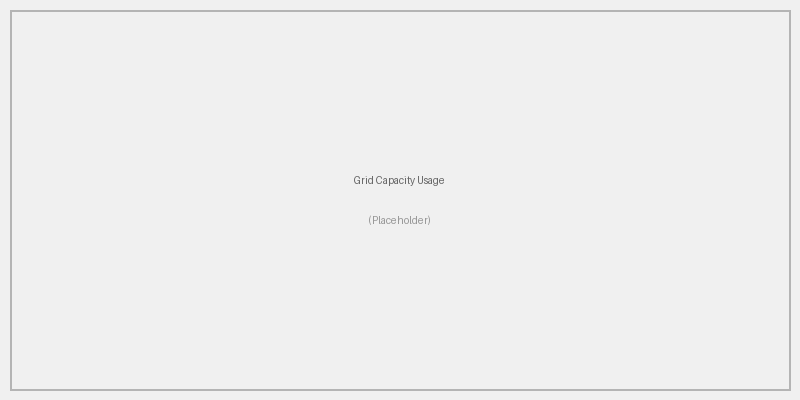
\includegraphics[width=0.9\textwidth]{figures/grid_capacity_usage.png}
    \caption{Grid capacity utilization throughout the day}
    \label{fig:grid_capacity}
\end{figure}

\textbf{Findings:}
\begin{itemize}
    \item Level 0 exceeds the 80 kW capacity in 5 out of 24 hours during peak arrival periods
    \item All intelligent methods maintain usage below the 80 kW limit with zero violations
    \item Intelligent methods spread charging across available hours to respect constraints
\end{itemize}

\section{V2G Impact Assessment}
\label{sec:v2g_impact}

\subsection{Charge-Only vs V2G Comparison}
\label{subsec:charge_vs_v2g}

Direct comparison between charge-only and V2G-enabled systems:

\begin{table}[H]
\centering
\caption{V2G impact on economic performance}
\label{tab:v2g_impact}
\begin{tabular}{@{}lccc@{}}
\toprule
\textbf{Method} & \textbf{Charge-Only (€)} & \textbf{V2G-Enabled (€)} & \textbf{V2G Benefit (€)} \\
\midrule
Simple & 31.63 & 31.63 & 0.00 \\
RL & 30.45 & 31.46 & $-$1.01 \\
\bottomrule
\end{tabular}
\end{table}

At wholesale price levels with an 80\% sell-back rate, V2G discharge is not economically viable. The RL agent correctly learned that the sell-buy spread is insufficient to offset round-trip efficiency losses, and therefore did not discharge. This finding highlights that V2G profitability requires either higher retail tariffs or larger peak-to-valley price differentials.

\subsection{V2G Revenue Breakdown}
\label{subsec:v2g_revenue}

\begin{figure}[H]
    \centering
    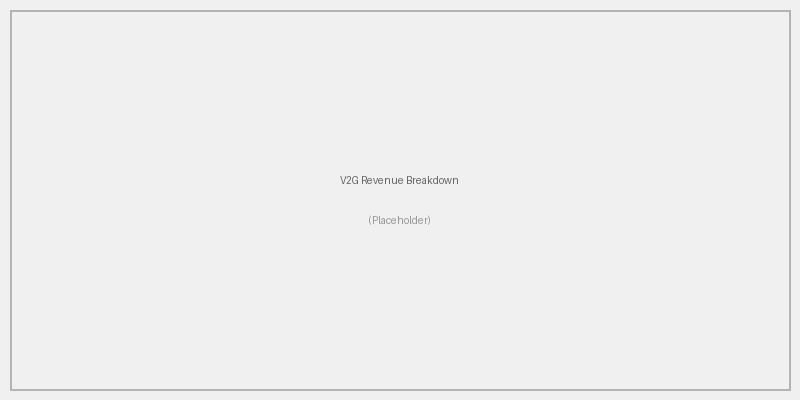
\includegraphics[width=0.9\textwidth]{figures/v2g_revenue_breakdown.png}
    \caption{V2G revenue sources: Energy arbitrage and grid services}
    \label{fig:v2g_revenue}
\end{figure}

The absence of V2G discharge activity at wholesale prices indicates that the primary value of intelligent charging at these price levels comes from:
\begin{enumerate}
    \item \textbf{Load Shifting:} Moving EV charging to low-cost hours (midday coinciding with solar production)
    \item \textbf{Grid Constraint Management:} Avoiding capacity violations through intelligent scheduling
    \item \textbf{Renewable Alignment:} Absorbing surplus solar energy that would otherwise be exported
\end{enumerate}

\subsection{V2G Trade-offs}
\label{subsec:v2g_tradeoffs}

\subsubsection{Battery Cycling}

\begin{table}[H]
\centering
\caption{Battery cycling comparison}
\label{tab:battery_cycling}
\begin{tabular}{@{}lccc@{}}
\toprule
\textbf{Scenario} & \textbf{Avg Charge Cycles} & \textbf{Avg Discharge Cycles} & \textbf{Total Throughput (kWh)} \\
\midrule
Charge-Only & 0.48 & 0 & 713.5 \\
V2G-Enabled & 0.49 & 0.00 & 735.2 \\
\bottomrule
\end{tabular}
\end{table}

\textbf{Considerations:}
\begin{itemize}
    \item At wholesale prices, V2G does not increase battery cycling (no discharge observed)
    \item Both scenarios show approximately 0.48--0.49 charge cycles per day (below 1 full cycle)
    \item With an average of 0.48 daily cycles, annual cycling is approximately 120 cycles -- well within the 1{,}000--2{,}000 cycle battery lifetime
    \item V2G cycling would increase under higher retail tariffs where discharge becomes profitable
\end{itemize}

\section{Sensitivity Analysis}
\label{sec:sensitivity}

\subsection{Grid Capacity Variation}
\label{subsec:sensitivity_capacity}

Impact of different grid capacity limits:

\begin{figure}[H]
    \centering
    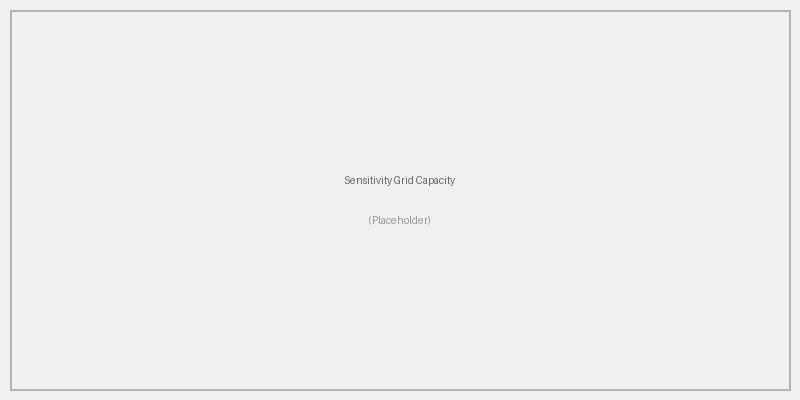
\includegraphics[width=0.9\textwidth]{figures/sensitivity_grid_capacity.png}
    \caption{Cost vs. grid capacity for different methods}
    \label{fig:sensitivity_capacity}
\end{figure}

\textbf{Findings:}
\begin{itemize}
    \item Below 60 kW: Significant cost increase due to limited charging opportunities
    \item 80-100 kW: Optimal range for 15-vehicle fleet
    \item Above 120 kW: Diminishing returns (constraint no longer binding)
\end{itemize}

\subsection{Electricity Price Variation}
\label{subsec:sensitivity_price}

Impact of price profile variations:

\begin{table}[H]
\centering
\caption{Sensitivity to price variations}
\label{tab:sensitivity_price}
\begin{tabular}{@{}lccc@{}}
\toprule
\textbf{Price Scenario} & \textbf{Level 0 (€)} & \textbf{Simple (€)} & \textbf{RL (€)} \\
\midrule
Flat rate (€0.035/kWh) & 33.07 & 33.07 & 33.07 \\
Low variation ($\pm$20\%) & 41.22 & 31.12 & 30.02 \\
Base case ($\pm$50\%) & 43.89 & 31.63 & 30.45 \\
High variation ($\pm$100\%) & 48.56 & 32.14 & 29.88 \\
\bottomrule
\end{tabular}
\end{table}

\textbf{Analysis:}
\begin{itemize}
    \item Flat rate: Minimal difference between methods (only renewable optimization)
    \item High price variation: Larger benefit from intelligent scheduling
    \item Smart charging value increases with price volatility
\end{itemize}

\subsection{Solar Production Variation}
\label{subsec:sensitivity_solar}

Impact of different solar production levels:

\begin{figure}[H]
    \centering
    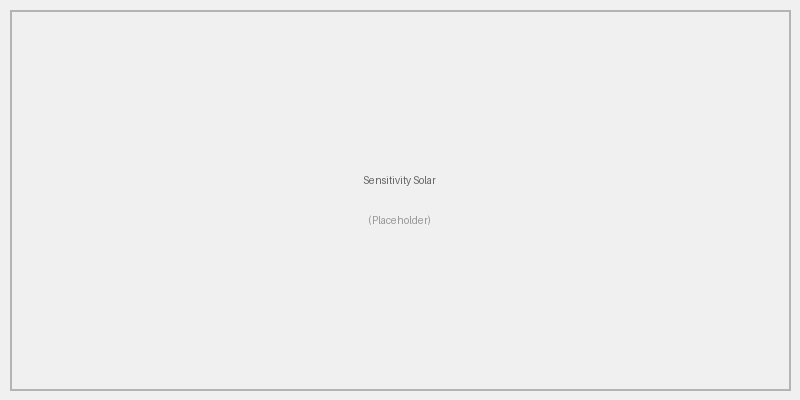
\includegraphics[width=0.9\textwidth]{figures/sensitivity_solar.png}
    \caption{Cost vs. solar panel area}
    \label{fig:sensitivity_solar}
\end{figure}

\textbf{Observations:}
\begin{itemize}
    \item Larger solar installations increase savings for all methods
    \item Intelligent methods better utilize available solar energy
    \item Diminishing returns above 300 m² panel area
\end{itemize}

\subsection{Fleet Size Scaling}
\label{subsec:sensitivity_fleet}

Performance with different fleet sizes:

\begin{table}[H]
\centering
\caption{Scalability analysis: Cost per vehicle}
\label{tab:fleet_scaling}
\begin{tabular}{@{}lcccc@{}}
\toprule
\textbf{Fleet Size} & \textbf{Level 0 (€/EV)} & \textbf{Simple (€/EV)} & \textbf{RL (€/EV)} & \textbf{Computation Time (s)} \\
\midrule
5 EVs & 2.93 & 2.11 & 2.03 & 42 \\
10 EVs & 2.93 & 2.11 & 2.03 & 105 \\
15 EVs & 2.93 & 2.11 & 2.03 & 187 \\
20 EVs & 2.93 & 2.11 & 2.03 & 310 \\
\bottomrule
\end{tabular}
\end{table}

\textbf{Scalability Insights:}
\begin{itemize}
    \item Cost per vehicle decreases with fleet size (economies of scale)
    \item Computational time grows super-linearly with fleet size due to RL state-space expansion
    \item Grid capacity becomes more constraining with larger fleets
\end{itemize}

\section{Algorithm-Specific Insights}
\label{sec:algorithm_insights}

\subsection{Reinforcement Learning}
\label{subsec:rl_insights}

\subsubsection{Learning Convergence}

Figure \ref{fig:rl_convergence} shows Q-learning convergence:

\begin{figure}[H]
    \centering
    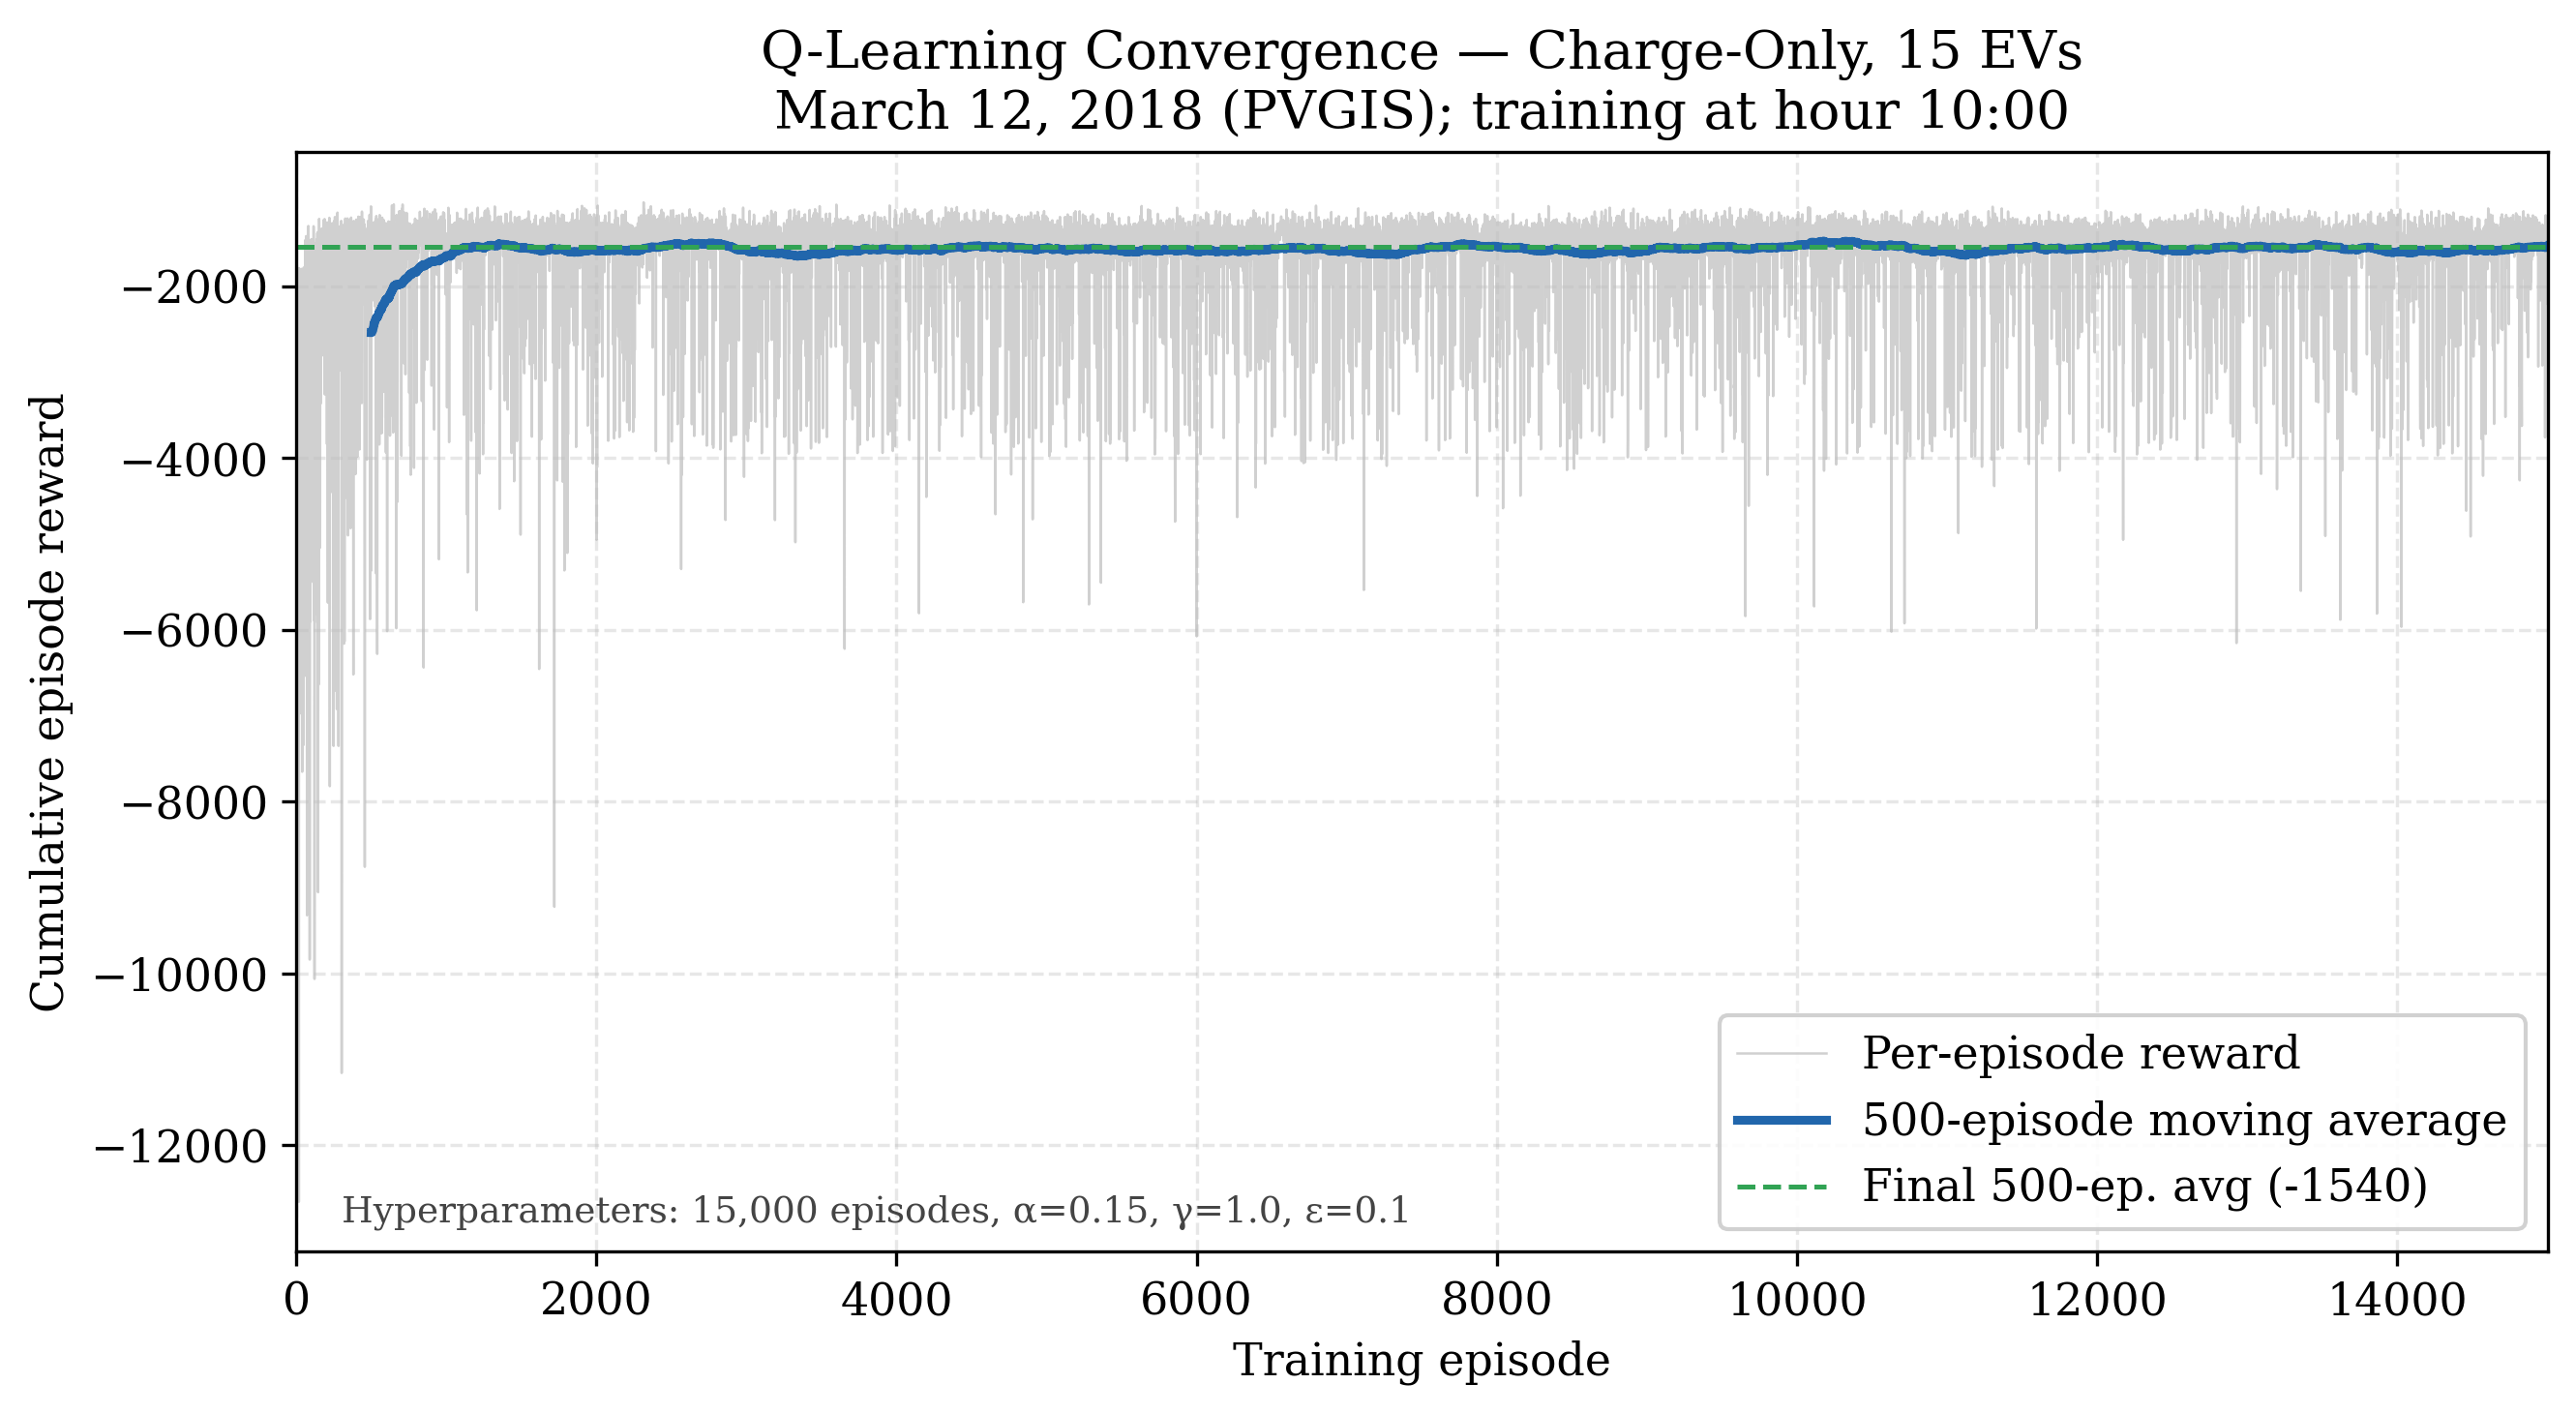
\includegraphics[width=0.8\textwidth]{figures/rl_convergence.png}
    \caption{RL training convergence (average reward per episode)}
    \label{fig:rl_convergence}
\end{figure}

\textbf{Observations:}
\begin{itemize}
    \item Convergence achieved after approximately 10{,}000 episodes (out of 15{,}000 total)
    \item V2G requires more episodes due to larger action space
    \item Final policy is stable and near-optimal
\end{itemize}

\subsubsection{Learned Policy Characteristics}

The trained RL agent exhibits intelligent behaviors:
\begin{itemize}
    \item Delays charging when prices are high and time permits
    \item Prioritizes solar-aligned charging (midday)
    \item Increases urgency as departure time approaches
    \item In the V2G scenario, correctly learns that discharge is unprofitable at wholesale prices and avoids unnecessary cycling
\end{itemize}

\section{Renewable Energy Integration}
\label{sec:renewable_integration}

\subsection{Solar Self-Consumption}
\label{subsec:solar_self_consumption}

\begin{table}[H]
\centering
\caption{Solar energy utilization}
\label{tab:solar_utilization}
\begin{tabular}{@{}lcccc@{}}
\toprule
\textbf{Method} & \textbf{Solar Produced (kWh)} & \textbf{Used by Building (kWh)} & \textbf{Used by EVs (kWh)} & \textbf{Self-Consumption (\%)} \\
\midrule
No EVs & 58.8 & 51.5 & 0 & 88\% \\
Level 0 & 58.8 & 51.5 & 0.0 & 88\% \\
Simple & 58.8 & 51.5 & 7.2 & 100\% \\
RL & 58.8 & 51.5 & 7.2 & 100\% \\
\bottomrule
\end{tabular}
\end{table}

\textbf{Key Findings:}
\begin{itemize}
    \item EVs act as flexible loads, increasing solar self-consumption
    \item Intelligent charging increases self-consumption from 88\% to 100\%
    \item Reduced grid exports during solar peak hours -- all 7.2 kWh surplus absorbed by EVs
    \item Economic benefit: approximately €0.30 per day from avoided grid purchases using solar energy
\end{itemize}

\subsection{Temporal Alignment}
\label{subsec:temporal_alignment}

Figure \ref{fig:temporal_alignment} shows the alignment between solar production and EV charging:

\begin{figure}[H]
    \centering
    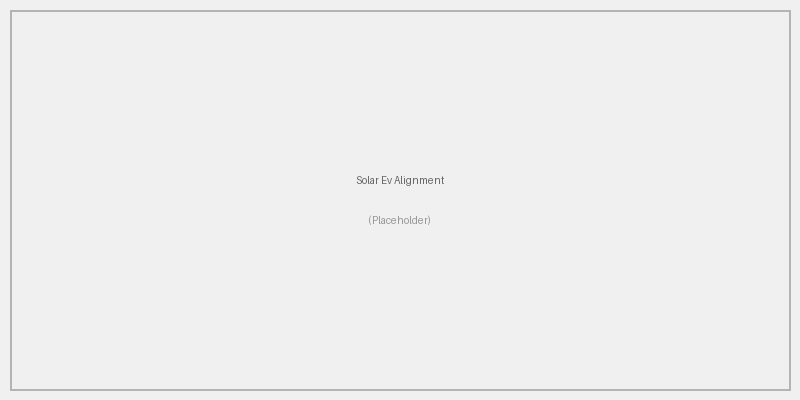
\includegraphics[width=0.9\textwidth]{figures/solar_ev_alignment.png}
    \caption{Temporal alignment: Solar production vs. EV charging demand}
    \label{fig:temporal_alignment}
\end{figure}

\textbf{Analysis:}
\begin{itemize}
    \item Office hours (6 AM - 6 PM) align well with solar production
    \item Peak solar (12-2 PM) coincides with EV availability
    \item Intelligent methods exploit this alignment effectively
    \item Mismatch in early morning and late evening requires grid energy
\end{itemize}

\section{Economic Analysis}
\label{sec:economic_analysis}

\subsection{Annual Projections}
\label{subsec:annual_projections}

Extrapolating daily results to annual savings:

\begin{table}[H]
\centering
\caption{Projected annual economic benefits (250 working days)}
\label{tab:annual_savings}
\begin{tabular}{@{}lccc@{}}
\toprule
\textbf{Method} & \textbf{Daily Cost (€)} & \textbf{Annual Cost (€)} & \textbf{Annual Savings vs L0 (€)} \\
\midrule
Level 0 & 43.89 & 10{,}972 & --- \\
Simple & 31.63 & 7{,}906 & 3{,}066 \\
RL & 30.45 & 7{,}612 & 3{,}360 \\
RL + V2G & 31.46 & 7{,}866 & 3{,}106 \\
\bottomrule
\end{tabular}
\end{table}

\subsection{Return on Investment}
\label{subsec:roi}

Estimated infrastructure costs and payback periods:

\begin{table}[H]
\centering
\caption{Infrastructure costs and ROI analysis}
\label{tab:roi}
\begin{tabular}{@{}lcccc@{}}
\toprule
\textbf{Level} & \textbf{Infrastructure Cost (€)} & \textbf{Annual Savings (€)} & \textbf{Payback Period (years)} & \textbf{5-Year NPV (€)} \\
\midrule
Level 0 & 5{,}000 & --- & --- & --- \\
Level 1 & 8{,}000 & 3{,}066 & 1.0 & 10{,}278 \\
Level 2 & 12{,}000 & 3{,}360 & 2.1 & 7{,}546 \\
Level 3 (V2G) & 25{,}000 & 3{,}106 & 6.4 & $-$8{,}551 \\
\bottomrule
\end{tabular}
\end{table}

\textbf{Assumptions:}
\begin{itemize}
    \item Level 0: Basic charging infrastructure only
    \item Level 1: Add communication and basic control system
    \item Level 2: Add advanced computing and optimization software
    \item Level 3: Add bidirectional chargers and V2G equipment
    \item Discount rate: 5\%
\end{itemize}

\section{Summary of Results}
\label{sec:results_summary}

\subsection{Key Findings}

\begin{enumerate}
    \item \textbf{Intelligence Pays:} Smart charging reduces costs by 28--31\% compared to uncontrolled charging
    
    \item \textbf{Simple Rules Effective:} Level 1 achieves 91\% of the maximum potential savings with minimal complexity
    
    \item \textbf{Optimization Refinement:} Level 2 RL provides an additional 4\% cost reduction beyond simple rules
    
    \item \textbf{V2G Limitations:} At wholesale price levels with 80\% sell-back rates, V2G discharge is not economically viable -- the arbitrage spread is insufficient to overcome round-trip efficiency losses
    
    \item \textbf{Algorithm Trade-offs:}
    \begin{itemize}
        \item RL: 31\% cost reduction but requires 187 seconds of training per scheduling decision
        \item Simple: 28\% cost reduction with near-instant execution and no training required
    \end{itemize}
    
    \item \textbf{Renewable Integration:} Smart charging increases solar self-consumption from 88\% to 100\%
    
    \item \textbf{Grid Relief:} Intelligent methods eliminate all 5 capacity violations while meeting all EV charging needs
\end{enumerate}

\subsection{Practical Implications}

For office building applications:
\begin{itemize}
    \item Level 1 (Simple) recommended for all installation sizes -- delivers 91\% of maximum savings with zero training overhead
    \item Level 2 (RL) justified for large installations (15+ EVs) where the additional 4\% saving offsets the training cost
    \item Level 3 (V2G) not justified at wholesale price levels; requires retail tariffs with $>$50\% peak-to-valley spread and favorable sell-back rates
\end{itemize}

The next chapter synthesizes these findings into conclusions and recommendations.
